% 
% Annual Cognitive Science Conference
% Sample LaTeX Paper -- Proceedings Format
% 

% Original : Ashwin Ram (ashwin@cc.gatech.edu)       04/01/1994
% Modified : Johanna Moore (jmoore@cs.pitt.edu)      03/17/1995
% Modified : David Noelle (noelle@ucsd.edu)          03/15/1996
% Modified : Pat Langley (langley@cs.stanford.edu)   01/26/1997
% Latex2e corrections by Ramin Charles Nakisa        01/28/1997 
% Modified : Tina Eliassi-Rad (eliassi@cs.wisc.edu)  01/31/1998
% Modified : Trisha Yannuzzi (trisha@ircs.upenn.edu) 12/28/1999 (in process)
% Modified : Mary Ellen Foster (M.E.Foster@ed.ac.uk) 12/11/2000
% Modified : Ken Forbus                              01/23/2004
% Modified : Eli M. Silk (esilk@pitt.edu)            05/24/2005
% Modified : Niels Taatgen (taatgen@cmu.edu)         10/24/2006
% Modified : David Noelle (dnoelle@ucmerced.edu)     11/19/2014
% Modified : Roger Levy (rplevy@mit.edu)     12/31/2018



%% Change "letterpaper" in the following line to "a4paper" if you must.

\documentclass[10pt,letterpaper]{article}

\usepackage{cogsci}
\usepackage{amsmath}
\usepackage{graphicx}
\usepackage{subcaption}

\cogscifinalcopy % Uncomment this line for the final submission 


\usepackage{pslatex}
\usepackage{apacite}
\usepackage{float} % Roger Levy added this and changed figure/table
                   % placement to [H] for conformity to Word template,
                   % though floating tables and figures to top is
                   % still generally recommended!

%\usepackage[none]{hyphenat} % Sometimes it can be useful to turn off
%hyphenation for purposes such as spell checking of the resulting
%PDF.  Uncomment this block to turn off hyphenation.


%\setlength\titlebox{4.5cm}
% You can expand the titlebox if you need extra space
% to show all the authors. Please do not make the titlebox
% smaller than 4.5cm (the original size).
%%If you do, we reserve the right to require you to change it back in
%%the camera-ready version, which could interfere with the timely
%%appearance of your paper in the Proceedings.



\title{The Art of (Recursive Bayesian) Persuasion}
 
\author{{\large \bf Samuel A. Barnett (samuelab@princeton.edu)} \\
  Department of Computer Science, 35 Olden Street \\
  Princeton, NJ 08540 USA}


\begin{document}

\maketitle


\begin{abstract}
Include no author information in the initial submission, to facilitate
blind review.  The abstract should be one paragraph, indented 1/8~inch on both sides,
in 9~point font with single spacing. The heading ``{\bf Abstract}''
should be 10~point, bold, centered, with one line of space below
it. This one-paragraph abstract section is required only for standard
six page proceedings papers. Following the abstract should be a blank
line, followed by the header ``{\bf Keywords:}'' and a list of
descriptive keywords separated by semicolons, all in 9~point font, as
shown below.

\textbf{Keywords:} 
AI; quantum; bitcoin; Elon Musk
\end{abstract}

\section{Introduction}
% Motivate the problem. Describe the strong and weak evidence effect. Say how you'll model these.

\section{Modeling Evidence Effects}
\subsection{World Model: The Stick Task}
% Introduce the notation and describe the objective of the stick task.
The stick task consists of a judge, and a set of speakers indexed by $I$. 
A sample of $N$ sticks whose lengths are given by
\begin{equation}
\mathcal{S}_N = \{ S_1, S_2, ..., S_N \}
\end{equation}
are drawn i.i.d.\ from the Uniform$[0,1]$ distribution and is fixed throughout
the task.\footnote{In practice, we use a discrete approximation to this distribution 
by modeling the sticks as being drawn uniformly from the set $\{ 0.025, 0.075, ..., 0.975\}$.} 

Each speaker observes the full sample before the task, and at each time step $t$ a speaker
$i$ (one per time step, taking it in turn) chooses one stick from the sample to reveal
to the judge. The speakers are not permitted to reveal a stick that has previously been shown to 
the judge. Notationally, the agent chooses action 
\begin{equation}
a_t^{(i)} \in \{s_1, s_2, ..., s_N\} \setminus \mathcal{A}_{t-1},
\end{equation}
where $s_i$ is the realization of random variable $S_i$ and $\mathcal{A}_{t-1}$ denotes the first
$t-1$ actions chosen. For simplicity, we let $\mathcal{A}_0 = \emptyset$.

At each time step $t$, the judge reasons about the sample mean of the sticks, 
$\bar{S} = \frac{1}{N} \sum_{n=1}^N S_n$.\footnote{It is assumed that the judge knows $N$, but only observes the stick values through the speakers' actions.}
In particular, the judge evaluates his posterior over whether the sample is `long' or `short', i.e., whether or not
$\bar{S	}_N \ge 0.5$. Hence, the relevant posterior for the judge at time step $t$ is
\begin{equation}
p( \bar{S}_N \ge 0.5 \ | \ \mathcal{A}_t ).
\end{equation}
Each speaker will have an incentive to select evidence that persuades the judge that the sample is
either long or short, or the speaker will be indifferent towards the outcome.

The task runs for a total of $T\le N$ time steps.

\subsection{Agent Models}
In the manner of Rational Speech Act (RSA) models, we model the agents as performing
recursive Bayesian inference about one another's beliefs. To capture both evidence effects,
we require four layers, which we divide into the `na\"ive' layers and the `pragmatic' layers.
The model is implemented in WebPPL, a probabilistic programming language that allows for
fast hierarchical inference in low-dimensional domains such as this one.

\subsubsection{Na\"ive Judge and Speaker}
The first layer, $J_0$, describes the na\"ive judge - this judge is na\"ive in the sense that he
does not model the speakers as having any incentives, and instead assumes that the actions are selected
uniformly from the available sample. Relabeling without loss of generality, the posterior of $J_0$ at time $t$ is given by
\begin{equation}
p_{J_0}( \bar{S}_N \ge 0.5 \ | \ S_1=s_1, S_2=s_2, ..., S_t=s_t).
\end{equation}

The second layer, $S_1$, describes the na\"ive speaker, whose choice about which stick to show
at time $t$ is represented as a posterior over the available sticks defined in reference to $p_{J0}$.
Importantly, each speaker has a bias $\beta$, where in our simulations we model the biases as being
in the range $\beta \in \{-10, -5, -2, 0, 2, 5, 10\}.$ This bias represents the incentive regarding the judge's
inference: a positive (resp. negative) bias entails that the speaker is incentivized to show sticks to the judge
that steer the judge towards the belief that the sample is long (resp. short).

To produce this behavior, the speaker samples a stick based on the soft-maximization of biased informativity
of that stick, taking into account the previous sticks shown:
\begin{equation}\label{S1}
p_{S_1} (a_t \ | \ \mathcal{A}_{t-1},\ \mathcal{S}_N) \propto \exp \bigl(\beta \cdot a_t \cdot p_{J_0} (\bar{S}_N \ge 0.5 \ | \ \mathcal{A}_{t-1} \cup \{a_t\} \bigr).
\end{equation}

Observe that, if $\beta = 0$, this entails that the speaker will sample the sticks uniformly based on the available
evidence, which is equivalent to the speaker being indifferent to the outcome.

\subsubsection{Pragmatic Judge and Speaker}
The pragmatic judge, $J_1$, performs a similar inference as $J_0$, though with one crucial difference: the judge
models each stick as having been sampled by a na\"ive speaker. To see how this is possible, observe that we can express
the action of speaker $i$ at time $t$ by the random variable 
\begin{equation}
	A_t^{(i)} \sim p_{S_1} (\cdot \ | \ \mathcal{A}_{t-1},\ \mathcal{S}_N),
\end{equation}
which is a categorical distribution computed by Equation~\ref{S1}. For ease of notation, we write the set
of observations of $S_1$ speakers
\begin{equation}
	\mathcal{A}'_T = \{ A_1^{(i_1)}=a_1^{(i_1)}, A_2^{(i_2)}=a_2^{(i_2)}, ..., A_T^{(i_T)}=a_T^{(i_T)}\}, 
\end{equation}
and let $\mathcal{A}'_0 = \emptyset$.

The posterior of $J_1$ can now be computed via Bayes' rule:
\begin{align*}
	p_{J_1} (\mathcal{S}_N \ | \ \mathcal{A}'_T) &\propto p(\mathcal{A}'_T \ | \ \mathcal{S}_N) p(\mathcal{S}_N) \\
	&=  p(\mathcal{S}_N) \prod_{t=1}^T p_{S_1}(A_t^{(i_t)}=a_t^{(i_t)} \ |  \mathcal{A}'_{t-1})
\end{align*}

Using the sum rule, we arrive at the relevant posterior, which in the case of discretized stick lengths is given by
\begin{equation}
	p_{J_1} ( \bar{S}_N \ge 0.5 \ | \ \mathcal{A}'_T ) = \sum_{\mathcal{S}_N \colon \bar{S}_N \ge 0.5} p_{J_1} (\mathcal{S}_N \ | \ \mathcal{A}'_T).
\end{equation}

We consider two distinct versions of the pragmatic judge: one in which he knows the biases of each agent in advance, and
one in which these biases are drawn, i.i.d., from a categorical prior over the aforementioned range of bias values. This is 
necessary as the weak and strong evidence effects demand the former and latter versions, respectively. 

We further divided the latter case into two by considering two possible priors: a flat prior over the bias range, and a `V-shaped' prior which down-weights 
the likelihood of neutrality.\footnote{Concretely, the V-shaped prior is given by the normalized probability vector $\frac{1}{29} [8, 4, 2, 1, 2, 4, 8]$.} 
We considered these two priors as, although the V-shaped prior better describes the context of the stick task, we wished to show 
that strong evidence effects were robust to our choice of prior. Factoring in uncertainty over the bias is then a matter of 
marginalizing over the possible bias settings using the sum rule.

The final layer, the pragmatic speaker $S_2$, is nearly identical to the na\"ive speaker $S_1$, except for the fact that
the pragmatic speaker performs soft-maximization based on $J_1$'s judgment, as opposed to $J_0$'s judgment:
\begin{equation}
p_{S_2} (a_t \ | \ \mathcal{A}_{t-1},\ \mathcal{S}_N) \propto \exp \bigl(\beta \cdot a_t \cdot p_{J_1} (\bar{S}_N \ge 0.5 \ | \ \mathcal{A}_{t-1} \cup \{a_t\} \bigr).
\end{equation}

This layer is only required to capture the strong evidence effects.

\section{Simulations}
\subsection{Simulation 1: Weak Evidence Effect}
%\begin{figure}[t!]
%\begin{center}
%\begin{subfigure}[t!]{0.2\textwidth}
%	\centering
%	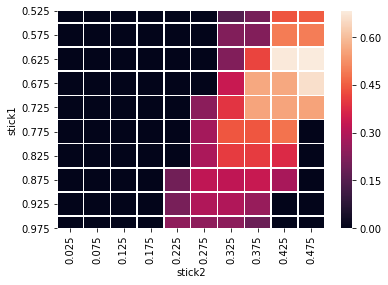
\includegraphics[width=\textwidth]{figures/wee3.png}
%	\label{fig:wee3}
%\end{subfigure}
%~
%\begin{subfigure}[t!]{0.2\textwidth}
%	\centering
%	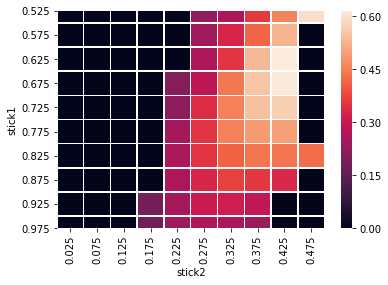
\includegraphics[width=\textwidth]{figures/wee4.png}
%	\label{fig:wee4}
%\end{subfigure}
%~
%\begin{subfigure}[t!]{0.2\textwidth}
%	\centering
%	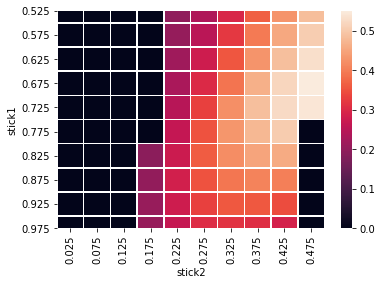
\includegraphics[width=\textwidth]{figures/wee5.png}
%	\label{fig:wee5}
%\end{subfigure}
%\end{center}
%\caption{This is a figure.} 
%\label{fig:wee}
%\end{figure}

\subsubsection{Set-Up}
In the first simulation, we captured the pragmatic judge's ability to capture the \textit{weak evidence effect}. We 
present the judge with one stick in turn from two speakers, whose biases are known to the judge and fixed at
$\beta_1 = 10, \beta_2 = -10$. We then contrast the na\"ive and pragmatic judge's posteriors over whether the
sample is long, having seen both sticks.

In this context, the weak evidence effect occurs when 

\subsubsection{Results}

\begin{figure}[H]
\begin{center}
\fbox{CoGNiTiVe ScIeNcE}
\end{center}
\caption{This is a figure.} 
\label{wee}
\end{figure}

\subsection{Simulation 2: Strong Evidence Effect for Speakers}
\subsubsection{Set-Up}
\subsubsection{Results}

\begin{figure}[H]
\begin{center}
\fbox{CoGNiTiVe ScIeNcE}
\end{center}
\caption{This is a figure.} 
\label{seeSpeaker}
\end{figure}

\begin{table}[H]
\begin{center} 
\caption{Sample table title.} 
\label{seeSpeakerTable} 
\vskip 0.12in
\begin{tabular}{ll} 
\hline
Error type    &  Example \\
\hline
Take smaller        &   63 - 44 = 21 \\
Always borrow~~~~   &   96 - 42 = 34 \\
0 - N = N           &   70 - 47 = 37 \\
0 - N = 0           &   70 - 47 = 30 \\
\hline
\end{tabular} 
\end{center} 
\end{table}

\subsection{Simulation 3: Strong Evidence Effect for Judges}
\subsubsection{Set-Up}
\subsubsection{Results}

\begin{figure}[H]
\begin{center}
\fbox{CoGNiTiVe ScIeNcE}
\end{center}
\caption{This is a figure.} 
\label{seeJudge}
\end{figure}

\section{Discussion and Future Work}


%\section{General Formatting Instructions}
%
%The entire content of a paper (including figures, references, and anything else) can be no longer than six pages in the \textbf{initial submission}. In the \textbf{final submission}, the text of the paper, including an author line, must fit on six pages. Up to one additional page can be used for acknowledgements and references.
%
%The text of the paper should be formatted in two columns with an
%overall width of 7 inches (17.8 cm) and length of 9.25 inches (23.5
%cm), with 0.25 inches between the columns. Leave two line spaces
%between the last author listed and the text of the paper; the text of
%the paper (starting with the abstract) should begin no less than 2.75 inches below the top of the
%page. The left margin should be 0.75 inches and the top margin should
%be 1 inch.  \textbf{The right and bottom margins will depend on
%  whether you use U.S. letter or A4 paper, so you must be sure to
%  measure the width of the printed text.} Use 10~point Times Roman
%with 12~point vertical spacing, unless otherwise specified.
%
%The title should be in 14~point bold font, centered. The title should
%be formatted with initial caps (the first letter of content words
%capitalized and the rest lower case). In the initial submission, the
%phrase ``Anonymous CogSci submission'' should appear below the title,
%centered, in 11~point bold font.  In the final submission, each
%author's name should appear on a separate line, 11~point bold, and
%centered, with the author's email address in parentheses. Under each
%author's name list the author's affiliation and postal address in
%ordinary 10~point type.
%
%Indent the first line of each paragraph by 1/8~inch (except for the
%first paragraph of a new section). Do not add extra vertical space
%between paragraphs.
%
%
%\section{First Level Headings}
%
%First level headings should be in 12~point, initial caps, bold and
%centered. Leave one line space above the heading and 1/4~line space
%below the heading.
%
%
%\subsection{Second Level Headings}
%
%Second level headings should be 11~point, initial caps, bold, and
%flush left. Leave one line space above the heading and 1/4~line
%space below the heading.
%
%
%\subsubsection{Third Level Headings}
%
%Third level headings should be 10~point, initial caps, bold, and flush
%left. Leave one line space above the heading, but no space after the
%heading.
%
%
%\section{Formalities, Footnotes, and Floats}
%
%Use standard APA citation format. Citations within the text should
%include the author's last name and year. If the authors' names are
%included in the sentence, place only the year in parentheses, as in
%\citeA{NewellSimon1972a}, but otherwise place the entire reference in
%parentheses with the authors and year separated by a comma
%\cite{NewellSimon1972a}. List multiple references alphabetically and
%separate them by semicolons
%\cite{ChalnickBillman1988a,NewellSimon1972a}. Use the
%``et~al.'' construction only after listing all the authors to a
%publication in an earlier reference and for citations with four or
%more authors.
%
%
%\subsection{Footnotes}
%
%Indicate footnotes with a number\footnote{Sample of the first
%footnote.} in the text. Place the footnotes in 9~point font at the
%bottom of the column on which they appear. Precede the footnote block
%with a horizontal rule.\footnote{Sample of the second footnote.}
%
%
%\subsection{Tables}
%
%Number tables consecutively. Place the table number and title (in
%10~point) above the table with one line space above the caption and
%one line space below it, as in Table~\ref{sample-table}. You may float
%tables to the top or bottom of a column, and you may set wide tables across
%both columns.
%
%\begin{table}[H]
%\begin{center} 
%\caption{Sample table title.} 
%\label{sample-table} 
%\vskip 0.12in
%\begin{tabular}{ll} 
%\hline
%Error type    &  Example \\
%\hline
%Take smaller        &   63 - 44 = 21 \\
%Always borrow~~~~   &   96 - 42 = 34 \\
%0 - N = N           &   70 - 47 = 37 \\
%0 - N = 0           &   70 - 47 = 30 \\
%\hline
%\end{tabular} 
%\end{center} 
%\end{table}
%
%
%\subsection{Figures}
%
%All artwork must be very dark for purposes of reproduction and should
%not be hand drawn. Number figures sequentially, placing the figure
%number and caption, in 10~point, after the figure with one line space
%above the caption and one line space below it, as in
%Figure~\ref{sample-figure}. If necessary, leave extra white space at
%the bottom of the page to avoid splitting the figure and figure
%caption. You may float figures to the top or bottom of a column, and
%you may set wide figures across both columns.
%
%\begin{figure}[H]
%\begin{center}
%\fbox{CoGNiTiVe ScIeNcE}
%\end{center}
%\caption{This is a figure.} 
%\label{sample-figure}
%\end{figure}
%
%
%\section{Acknowledgments}
%
%In the \textbf{initial submission}, please \textbf{do not include
%  acknowledgements}, to preserve anonymity.  In the \textbf{final submission},
%place acknowledgments (including funding information) in a section \textbf{at
%the end of the paper}.
%
%
%\section{References Instructions}
%
%Follow the APA Publication Manual for citation format, both within the
%text and in the reference list, with the following exceptions: (a) do
%not cite the page numbers of any book, including chapters in edited
%volumes; (b) use the same format for unpublished references as for
%published ones. Alphabetize references by the surnames of the authors,
%with single author entries preceding multiple author entries. Order
%references by the same authors by the year of publication, with the
%earliest first.
%
%Use a first level section heading, ``{\bf References}'', as shown
%below. Use a hanging indent style, with the first line of the
%reference flush against the left margin and subsequent lines indented
%by 1/8~inch. Below are example references for a conference paper, book
%chapter, journal article, dissertation, book, technical report, and
%edited volume, respectively.

\nocite{ChalnickBillman1988a}
\nocite{Feigenbaum1963a}
\nocite{Hill1983a}
\nocite{OhlssonLangley1985a}
% \nocite{Lewis1978a}
\nocite{Matlock2001}
\nocite{NewellSimon1972a}
\nocite{ShragerLangley1990a}


\bibliographystyle{apacite}

\setlength{\bibleftmargin}{.125in}
\setlength{\bibindent}{-\bibleftmargin}

\bibliography{CogSci_Template}


\end{document}
